\section{Field Reports from Commercial App Developers}
The research includes field reports from developers of three distinct commercial Android apps. Each uses mobile analytics in their regular software development practices.

\subsection{Characteristics of the commercial apps}

\begin{itemize}
    \item Technologies
    \item Analytics available to the team
    \item Development priorities for their use of analytics
\end{itemize}

\subsection{Moonpig}


\subsection{Moodspace}


\subsection{Local Halo}
MUST-DO complete this sub-section on Local Halo.

\begin{table}[htbp!]
    \centering
    \small
    \begin{tabular}{ll}
       Question &Answer  \\
       Website &\url{https://www.localhalo.com/} \\
       Founded &2018\\
       Business Domain &Digital neighbourhood groups in UK.\\
       Business type &Startup \\
       Technologies  &React Native \\
       Analytics Available &Sentry, Mixpanel, Google Play Console \\
       Development Practices &Cross-platform development
    \end{tabular}
    \caption{Case Study Overview: Localhalo}
    \label{tab:local_halo_anaytics_overview}
\end{table}

\subsubsection{Experiences of using mobile analytics}
Localhalo incorporate two analytics libraries into their cross-platform mobile application: sentry for crash reporting and mixpanel for business-oriented usage analytics. For their Android app they also have access to Google Play Console.

They experience numerous crashes reported by Sentry, which occur within the React Native runtime environment. Sentry provides email alerts to the development team together with summary reports, (Figure~\ref{fig:localhalo-sentry-weekly-report-21-sep-2020} is example for the period~\nth{14} to~\nth{21} September 2020), and online access to their analytics.

A release in March 2020 had a high crash rate for the production release of their Android app. The top crash cluster was for:

\texttt{java.lang.RuntimeExceptionhost.exp.exponent.experience.a\$b.run}. 

This was traced to a problem in the expo library they used in the app~\url{https://github.com/expo/expo/issues/5839}. In that issue several developers for different Android apps provide data from Google Play Console confirming they also receive similar crash clusters. The cause has not yet been definitively traced or addressed, however for the LocalHalo app the crashes stopped being reported once a new release of the Android app, release 1.3.0, was released around \nth{6} April 2020.

\begin{figure}[htbp!]
    \centering
    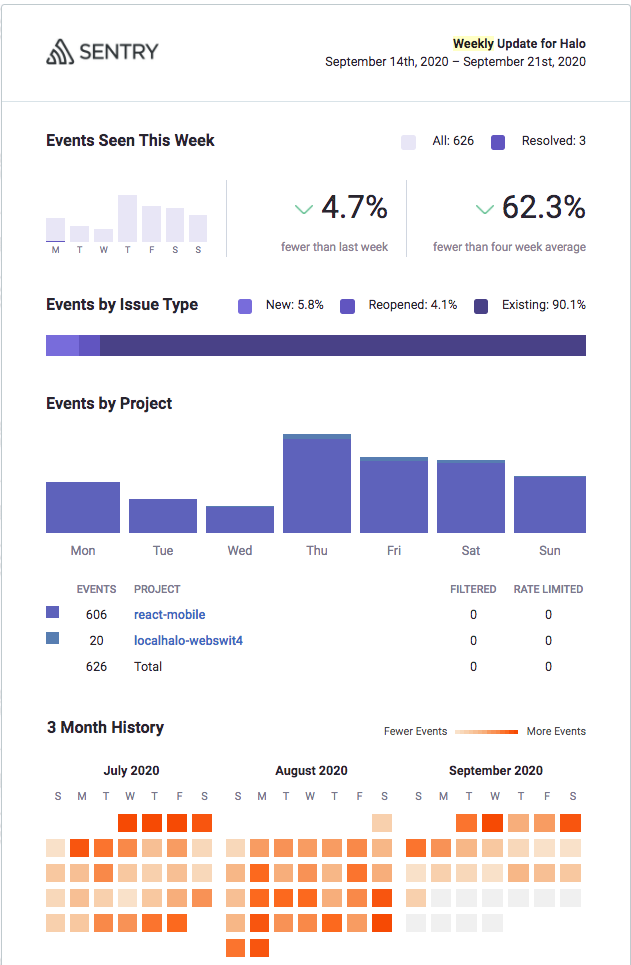
\includegraphics[width=9cm]{images/localhalo/sentry-weekly-report-21-Sep-2020.png}
    \caption{LocalHalo: Sentry weekly report 14 - 21 September 2020}
    \label{fig:localhalo-sentry-weekly-report-21-sep-2020}
\end{figure}

\textbf{Sentry}

MUST-DO Check in Sentry for the various types of error. How actively are the development team reading, reviewing and addressing crashes being reported? 

\begin{figure}[htbp!]
\centering
\begin{minipage}{.5\textwidth}
  \centering
  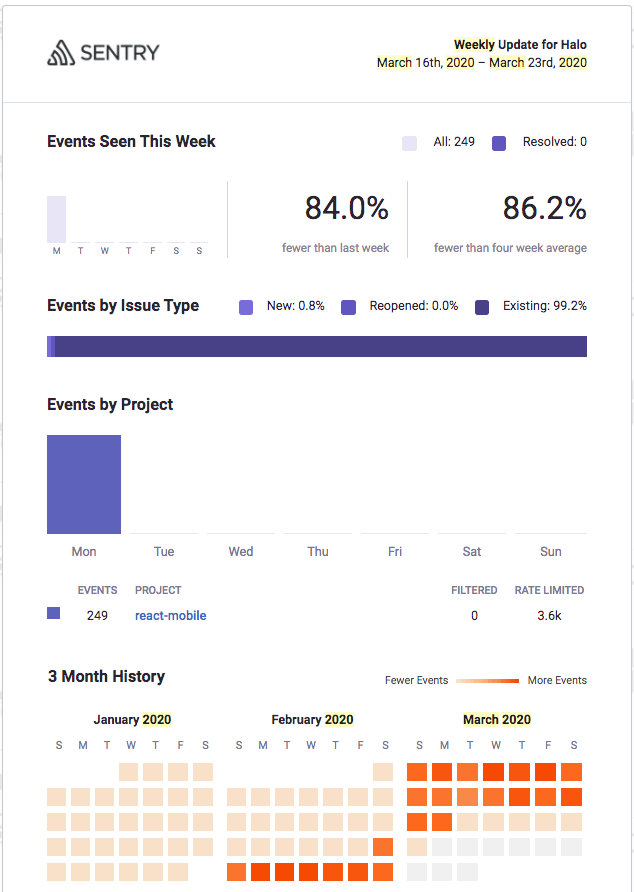
\includegraphics[width=.8\linewidth]{images/localhalo/sentry-weekly-report-16-mar-2020.png}
  \captionof*{figure}{\nth{16} -~\nth{22} March 2020}
  \label{fig:localhalo-sentry-weekly-report-16-mar-2020}
\end{minipage}%
\begin{minipage}{.5\textwidth}
  \centering
  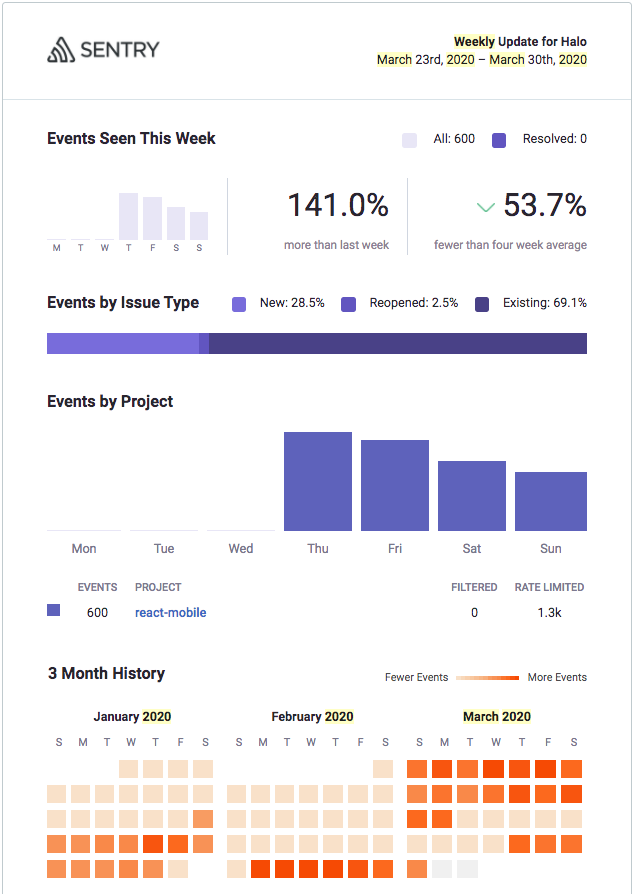
\includegraphics[width=.8\linewidth]{images/localhalo/sentry-weekly-report-23-mar-2020.png}
  \captionof*{figure}{\nth{23} -~\nth{29} March 2020}
  \label{fig:localhalo-sentry-weekly-report-23-mar-2020}
\end{minipage}
    \caption{Missing data reported in Sentry}
    \label{fig:sentry-missing-data-march-2020}
\end{figure}

\begin{comment}


\begin{figure}[htbp!]
    \centering
    %\subfigure[]{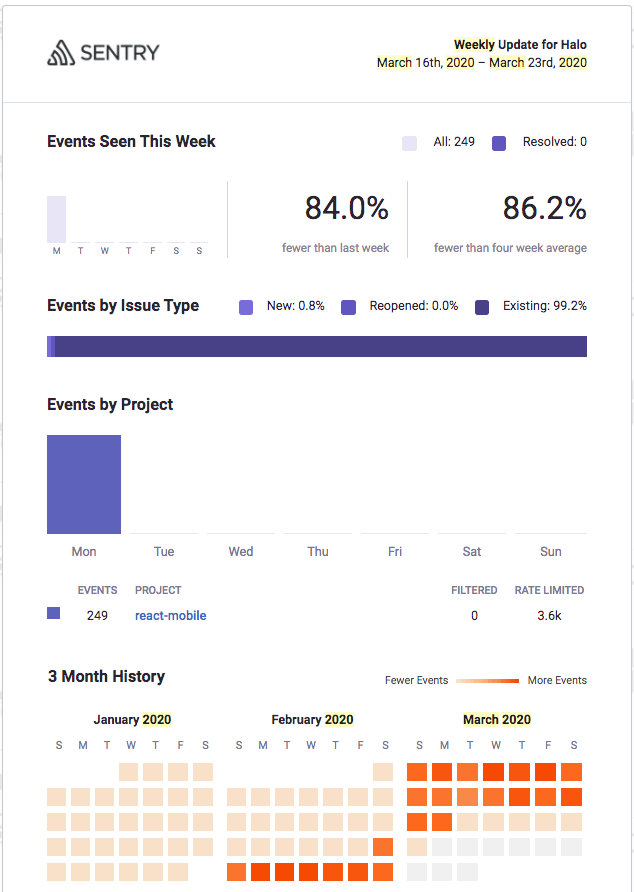
\includegraphics[width=0.4\textwidth]{images/localhalo/sentry-weekly-report-16-mar-2020.png}\caption{\nth{16} -~\nth{22} March 2020}\label{localhalo-sentry-weekly-report-16-mar-2020}}
    \subfigure[]{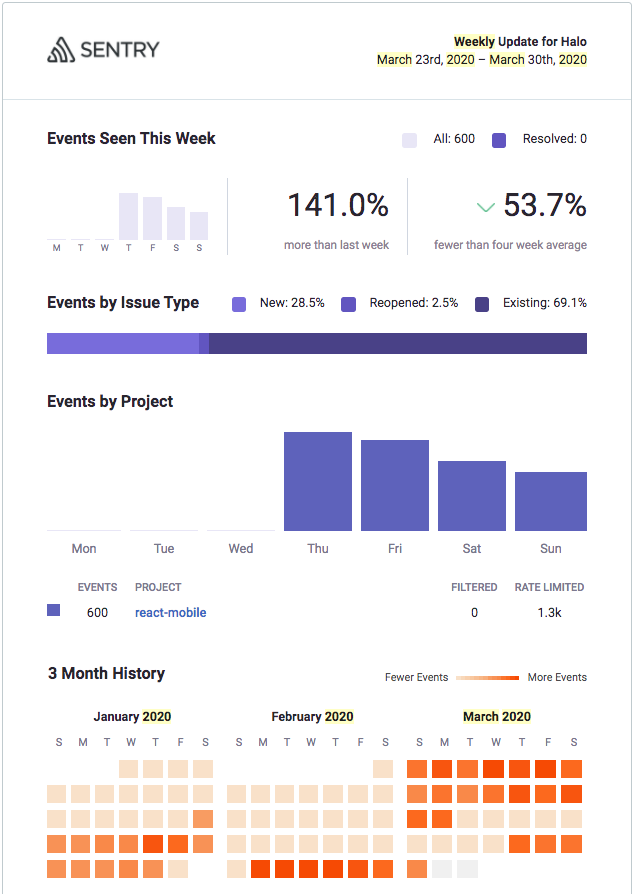
\includegraphics[width=0.4\textwidth]{images/localhalo/sentry-weekly-report-23-mar-2020.png}%\caption{\nth{23} -~\nth{29} March 2020}%\label{localhalo-sentry-weekly-report-23-mar-2020}
    }
    \caption{Missing data reported in Sentry}
    \label{fig:sentry-missing-data-march-2020}
\end{figure}
\end{comment}

%TODO fix the layout of the above figures: try: https://tex.stackexchange.com/questions/37581/latex-figures-side-by-side/37597#37597
Data missing from reports from~\nth{17} March to~\nth{25} March 2020 which affected the statistics around the time of the crashes related to Expo. Figure~\ref{fig:sentry-missing-data-march-2020} illustrates the gap across the two weekly reports. 

SHOULD-DO Consider summarising the crash totals per week. 

\textbf{MUST-DO} write up what we learn from the localhalo case study. external libraries can adversely affect the reliability of apps. Even small development teams can and do use multiple mobile analytics libraries. What can developers learn from the various reports provided by Sentry? How does cross-platform development in react-native affect the app reliability? are there crashes that only occur on Android or iOS? What's the correlation between crashes reported in Android Vitals and Sentry?


\subsection{Summary of Field Reports}
Active and ongoing use. 